\documentclass{article}
\usepackage[utf8]{inputenc}
\usepackage[T1]{fontenc}
\usepackage{graphicx}
\usepackage{hyperref}
\usepackage{geometry}
\geometry{margin=1in}

\title{HE A  776}
\date{Encyclopaedia Britannica (1771)}

\begin{document}
\maketitle

\section*{Historical source}
\textbf{Entry ID:} \texttt{entry-he-a-776-1032} \\
\textbf{Volume ID:} 144850367 \\
\textbf{Character Count:} 2283

\subsection*{Extracted Text}
What the doctor thus calculates, from deposition, with regard to mandind, he actually experimented op-on horfes, dogs, fallow-does, cz, by fixing tubes, in<y\_0.1734><class\_Text>

<x\_0.5459><y\_0.0625>cerifices opened in their veins and arteries ; by obfer-ving into federal heights, or which the blood rode in these tubes, as they lay on the ground, y and by mea- firing the capacities of the ventricles of the heart, and orifice of the arteries. And, that the reader may the more readily compare the faid eliminates together, he has given a table of them, ranged in the following order.

\textbackslash{}begin\{tabular\}\{ccccccccccc\}
**The feeral animals.** \& **Weight of each.** \& **Height of the blood in the tube from the gui- urine.** \& **Capacity of the left ventricle of the heart.** \& **Area of the orifice of the aorta.** \& **Velocity of the blood in the sorta.** \& **Welocity of the blood in the sorta.** \& **Flows.** \& **How much in a minute** \& **Weight of the blood fur- flined by the left ventricle contracting.** \& **Area of transferfe fiction of defending aorta.** \& **Area of the transferfe fiction of defending aorta.**\textbackslash{}\textbackslash{}
 \& Pounds, Ounces. \& Inches. \& Retelaches. \& Cubicinches \& Square inches. \& Pete andiae circa in minute. \& Minutes. \& Pounds. \& Pounds. \& No of pullies in a minute. \& Square inches.\textbackslash{}\textbackslash{}
Man \& 160 \& On drain- ing. \& 7 6 \& 1.659 \& 3.318 \& 0.4187 \& 56.55 \& 34.18 \& 34.38 \& 51.5 \& \textbackslash{}\textbackslash{}
Horfe 1th. 2d. 3d. \& 12 5 \& 9 8 \& 8 9 \& 10 2.5 \& 1.036 \& 86.85 \& 60 88 \& 13.75 \& 113.22 \& 86 38 \& 0.369\textbackslash{}\textbackslash{}
Ox \& 835 1600 \& 12 5 \& 9 6 \& 10 1.539 \& 86.95 \& 76.95 \& 18.14 \& 113.22 \& 86 38 \& 0.677 0.912 \& 0.84\textbackslash{}\textbackslash{}
Sheep Doe \& 91 \& 5† \& 9 6 \& 1.85 \& 0.172 0.476 \& 174.5 \& 20 \& 4.593 \& 36.56 \& 50 0.984 \& 0.07 0.012\textbackslash{}\textbackslash{}
Dogs ift. \& 52 24 \& 5 6 \& 6 8 8 \& 1.172 \& 0.196 \& 144.77 \& 11.9 \& 4.34 \& 33.61 \& 97 \& 0.106 0.034\textbackslash{}\textbackslash{}
2d. 3d. 3d. \& 18 5 \& 5 7 \& 8 8 \& 0.185 \& 0.118 \& 130 \& 7.8 \& 2.3 \& 19.8 \& 11.1 \& 0.07 0.022 0.009\textbackslash{}\textbackslash{}
4th. \& 12 8 \& 4 \& 8 3 \& 0.633 \& 0.101 \& 120 \& 6.7 \& 1.85 \& 11.1 \& 0.061 \& 0.015 0.007\textbackslash{}\textbackslash{}
\textbackslash{}end\{tabular\}

tery of a man, and that the inward area of the left ventricle of his heart is equal to fifteen figures under; their multiplied inn =+1 for, give 13 to cubicinches of blood, which prefix on that ventricle, when it drift begins to control, a weight equal to 15 y.g pounds.

\subsection*{Matched Wikipedia Article}
\textbf{Title:} Inward investment \\
\textbf{Page ID:} 347261 \\
\textbf{Revision ID:} 1352223370 \\
\textbf{URL:} \url{https://en.wikipedia.org/wiki/Inward\_investment}


\section*{Source record}
\begin{itemize}
\item \textbf{Dataset:} \texttt{NationalLibraryOfScotland/encyclopaedia\_britannica\_illustrated}
\item \textbf{Dataset Revision:} \texttt{309f765b1ecc83e0a7f7762e44b4a927a7555443}
\item \textbf{Page ID:} \texttt{britannica:309f765b1ecc83e0a7f7762e44b4a927a7555443:train:1032} \\
  \textbf{Filename:} \texttt{page-1032-e28420685b47.jpg} \\
  \textbf{Row Index:} 1032 \\
  \textbf{SHA256:} \texttt{e28420685b477a2b...}
\end{itemize}

\begin{figure}[h]
\centering
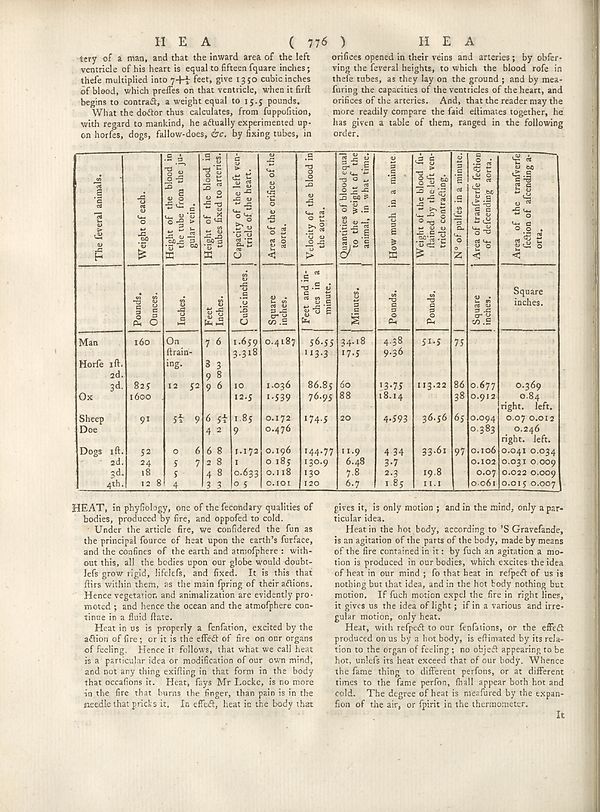
\includegraphics[width=0.85\textwidth]{../scans/page-1032-e28420685b47.jpg}
\caption*{Source scan: \texttt{page-1032-e28420685b47.jpg}}
\end{figure}

\end{document}
